\documentclass{article}

\usepackage{float}
\usepackage{color}
\usepackage{cleveref}
\usepackage{csvsimple}
\usepackage{graphicx}
\usepackage{longtable}
\usepackage{booktabs}

\makeatletter
\newcommand*{\centerfloat}{%
  \parindent \z@
  \leftskip \z@ \@plus 1fil \@minus \textwidth
  \rightskip\leftskip
  \parfillskip \z@skip}
\makeatother

\begin{document}

\section{Fixed versus growing seed words}

Here, we compare three situations:

\begin{itemize}
    \item \texttt{fixed seeds}: throughout the analysis, only access the seed
        words available in 1800;
    \item \texttt{varying seeds}: in each decade, evaluate the model on all
        seed words available then;
    \item \texttt{restricted seeds}: in each decade, use all seed words
        available in that decade to make predictions, \textit{but only measure
        predictive accuracy over the seed words available in 1800}.
\end{itemize}

The reason to look at the third, unorthodox-looking option is to distinguish
between two possible reasons for degraded performance in more recent decades:
1) more recently-available words are harder, and 2) more recently-available
words add noise to the model and affect previously-correct predictions.

\Cref{fig:seeds-categorization,fig:seeds-null,fig:seeds-polarity}
suggest that words whose embeddings are only available more recently are,
in fact, more difficult to classify.

\begin{figure}[H]
    \centerfloat
    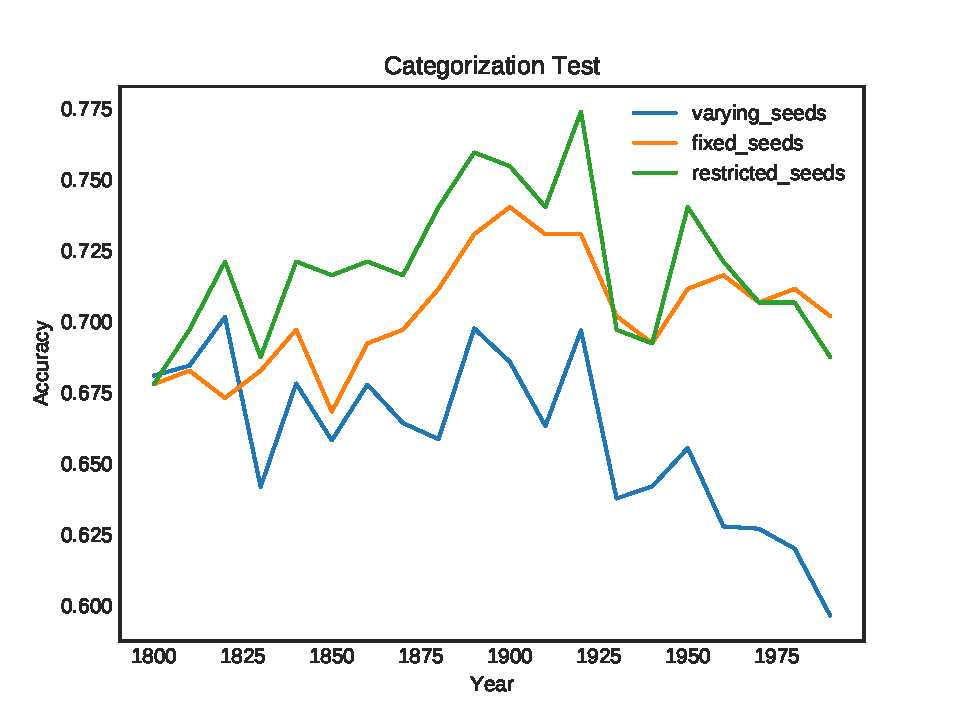
\includegraphics[width=1.5\linewidth]{classification-centroid-fixed-varying-restricted-seeds/results_categorization_test.pdf}
    \caption{Categorization accuracy for different seed word regimes}
    \label{fig:seeds-categorization}
\end{figure}

\begin{figure}[H]
    \centerfloat
    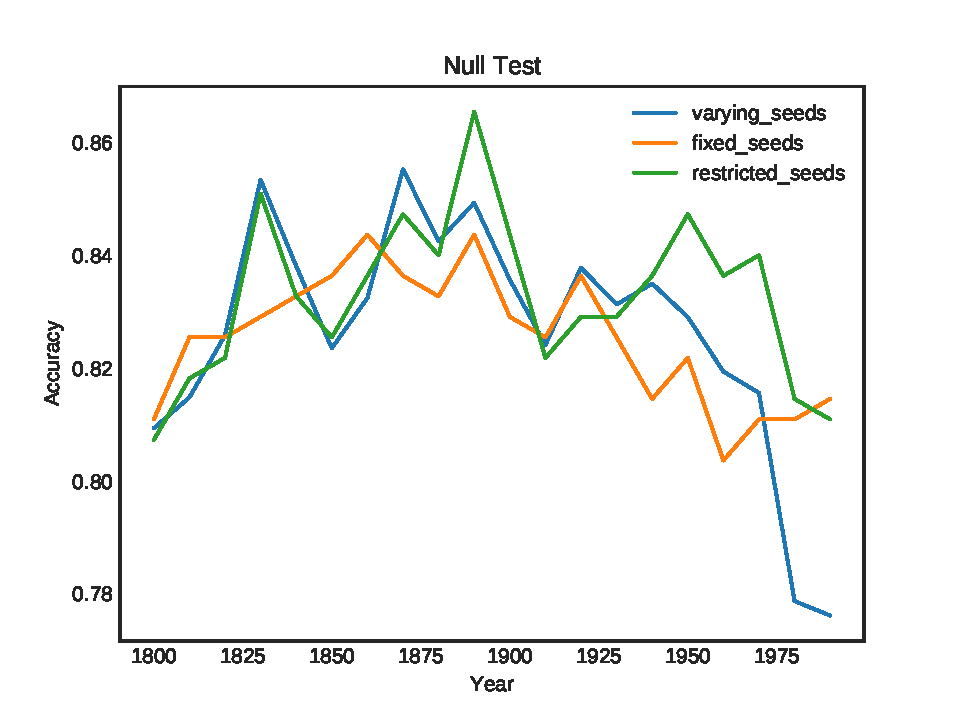
\includegraphics[width=1.5\linewidth]{classification-centroid-fixed-varying-restricted-seeds/results_null_test.pdf}
    \caption{Null test accuracy for different seed word regimes}
    \label{fig:seeds-null}
\end{figure}

\begin{figure}[H]
    \centerfloat
    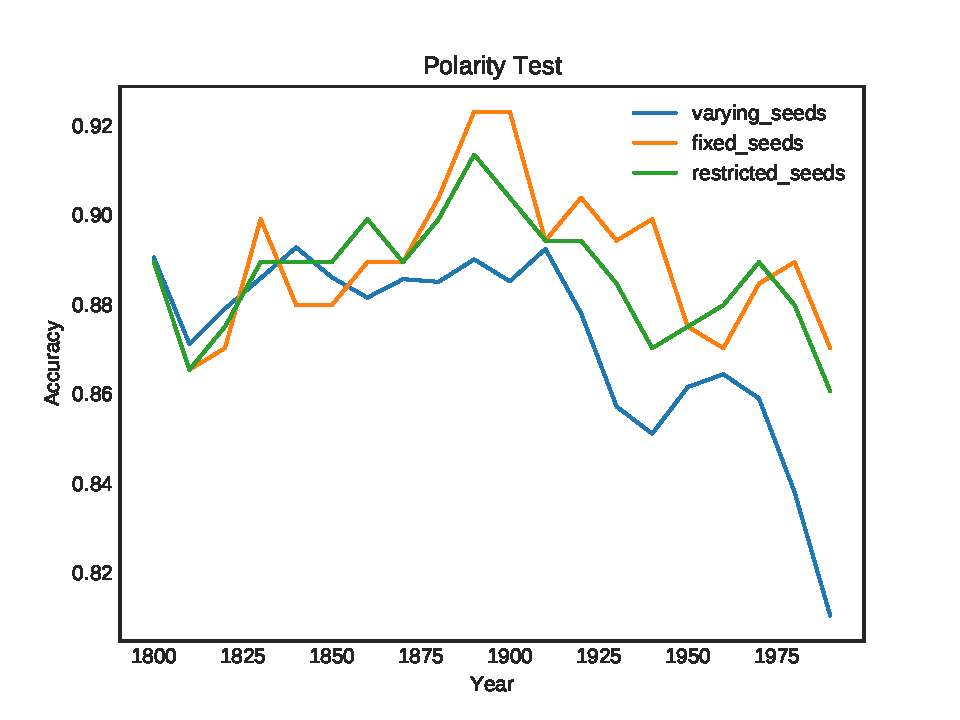
\includegraphics[width=1.5\linewidth]{classification-centroid-fixed-varying-restricted-seeds/results_polarity_test.pdf}
    \caption{Polarity test accuracy for different seed word regimes}
    \label{fig:seeds-polarity}
\end{figure}

\section{FDA + centroid classifier}

We repeat the classification tests using the centroid method, but pre-process
word embeddings in each decade by applying FDA dimension reduction to them.

More precisely, before predicting each seed word $s$ in the leave-one-out
procedure, we apply FDA to the set of all seed words \textit{except for $s$},
and use the coefficients obtained to project $s$ into the same space. Then,
we classify $s$ as before in the reduced space.

Since we now have 11 categories in total (10 moral categories along with a
neutral category), we perform FDA over 10 dimensions (instead of 9).
We apply shrinkage coefficient $0.5$, and use the \texttt{eigen} solver of
\texttt{scikit-learn}.

\begin{figure}[H]
    \centerfloat
    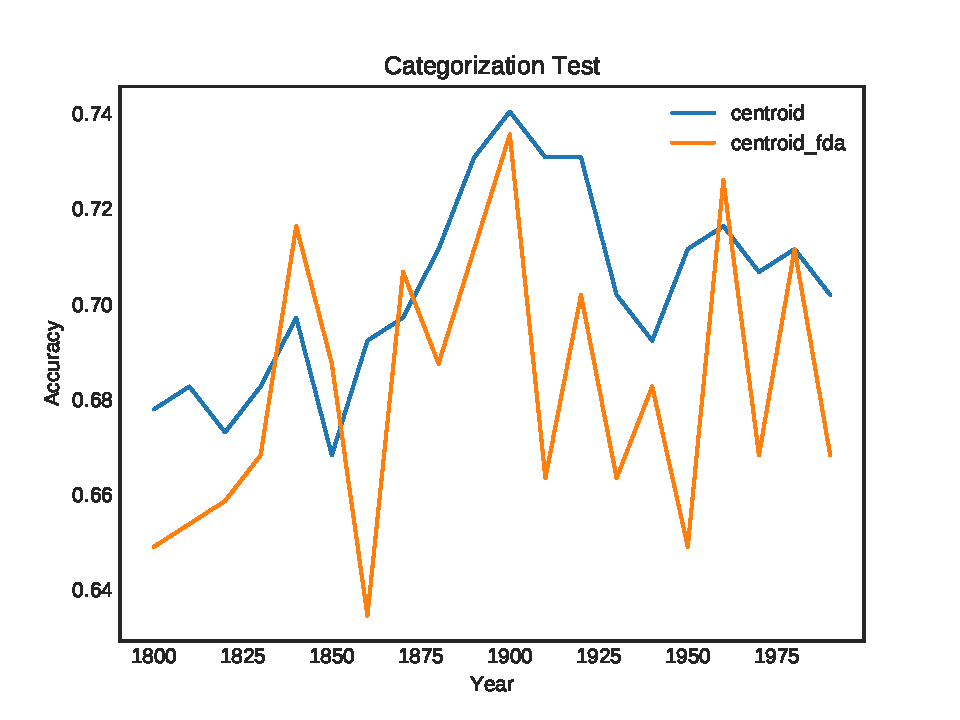
\includegraphics[width=1.5\linewidth]{centroid-fda-vs-not-fixed-seeds/results_categorization_test.pdf}
    \caption{Categorization accuracy with centroid and FDA+centroid methods}
    \label{fig:fda-categorization}
\end{figure}

\begin{figure}[H]
    \centerfloat
    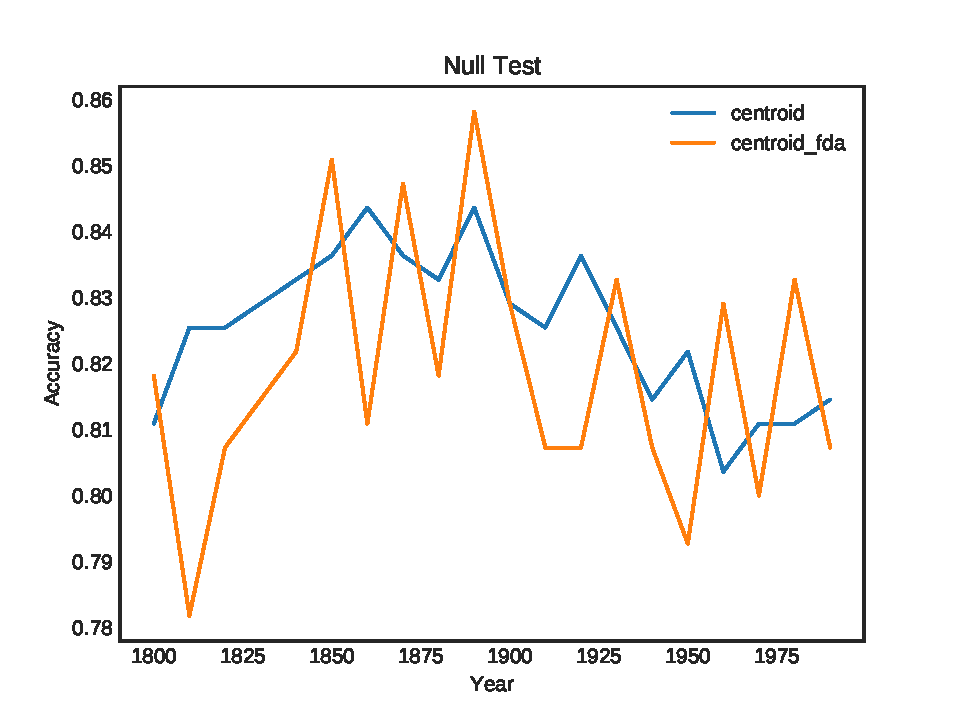
\includegraphics[width=1.5\linewidth]{centroid-fda-vs-not-fixed-seeds/results_null_test.pdf}
    \caption{Null test accuracy with centroid and FDA+centroid methods}
    \label{fig:fda-null}
\end{figure}

\begin{figure}[H]
    \centerfloat
    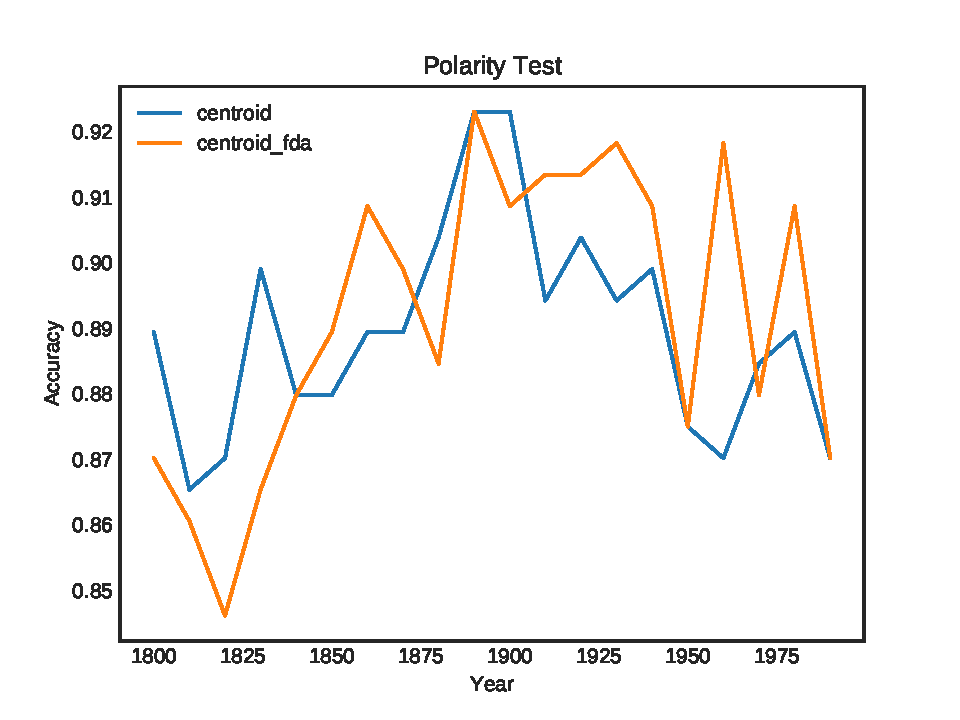
\includegraphics[width=1.5\linewidth]{centroid-fda-vs-not-fixed-seeds/results_polarity_test.pdf}
    \caption{Polarity test accuracy with centroid and FDA+centroid methods}
    \label{fig:fda-polarity}
\end{figure}

\Cref{fig:fda-categorization,fig:fda-null,fig:fda-polarity} show classification
accuracy in the \texttt{fixed seeds} regime (same seed words as 1800) for both
methods. Applying FDA prior to classification does not seem to systematically
improve predictive accuracy.

\section{Confusion matrices}

\Cref{fig:confusion-categorization-fixed,fig:confusion-categorization-varying,fig:confusion-null-fixed,fig:confusion-null-varying,fig:confusion-polarity-fixed,fig:confusion-polarity-varying}
show confusion matrices for each classification test under each of the
fixed seeds and varying seeds regimes, both of which display similar patterns.

The category \texttt{-loyalty} seems particularly challenging, and seems to
be confused with \texttt{-sanctity}. The number of available seed words for
each category may play a contributing role (see \Cref{tab:sizes}), but it is not
yet clear how significant this factor is versus other potential causes.

\textcolor{blue}{NOTE:}
One possible idea is to artificially rebalance classes, at least somewhat,
and see whether this anomaly improves. I (RF) suspect not, and that the
problem is semantic in nature.

\textcolor{blue}{NOTE:}
Once kernel density procedures have finished, we will be able to see how
that model compares in this particular challenging case.

\textcolor{red}{TODO:}
Consider enlarging neutral seed word set to match positive + negative words,
and whether to do so pre- or post- embedding filtering (bias?).

\begin{figure}[H]
    \centerfloat
    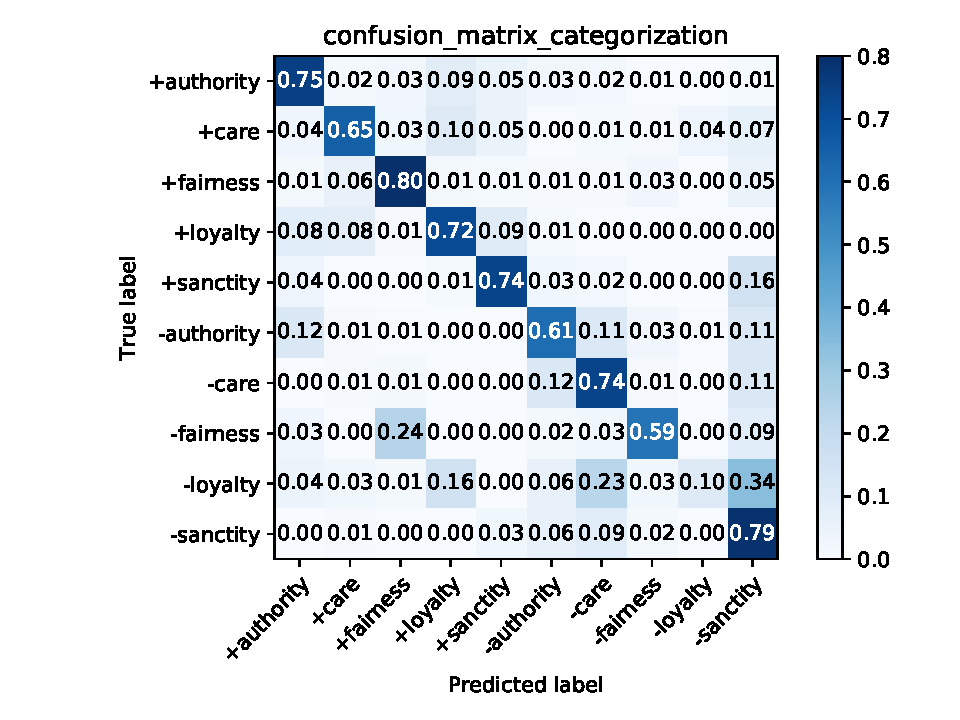
\includegraphics[width=1.5\linewidth]{confusion-matrix-centroid-fixed-seeds/confusion_matrix_categorization.pdf}
    \caption{Categorization confusion matrix for fixed seeds.}
    \label{fig:confusion-categorization-fixed}
\end{figure}

\begin{figure}[H]
    \centerfloat
    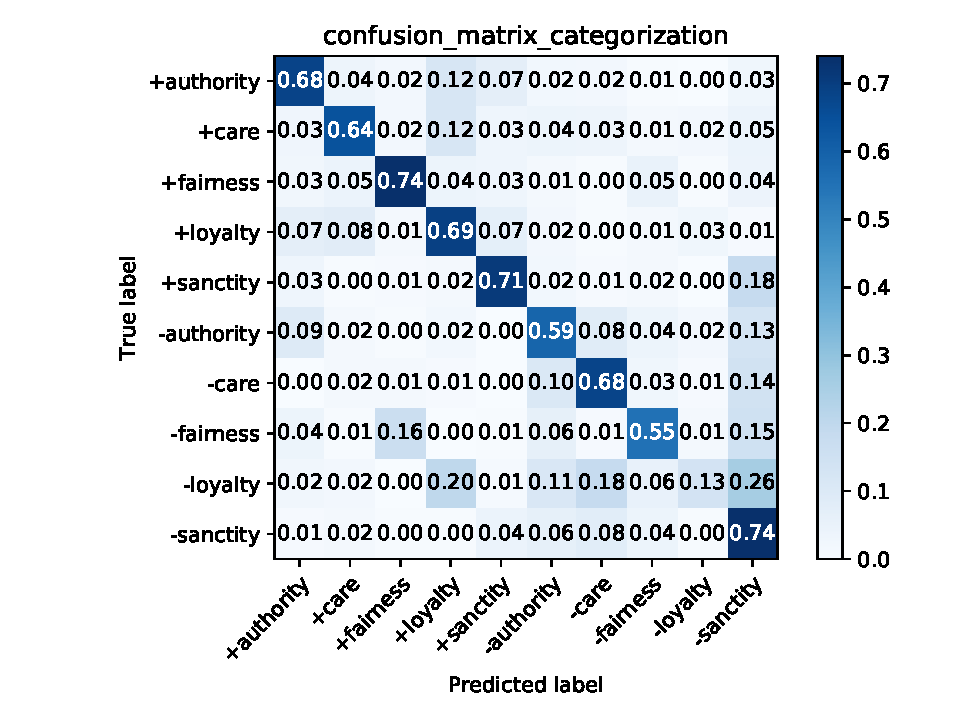
\includegraphics[width=1.5\linewidth]{confusion-matrix-centroid-varying-seeds/confusion_matrix_categorization.pdf}
    \caption{Categorization confusion matrix for varying seeds.}
    \label{fig:confusion-categorization-varying}
\end{figure}

\begin{figure}[H]
    \centerfloat
    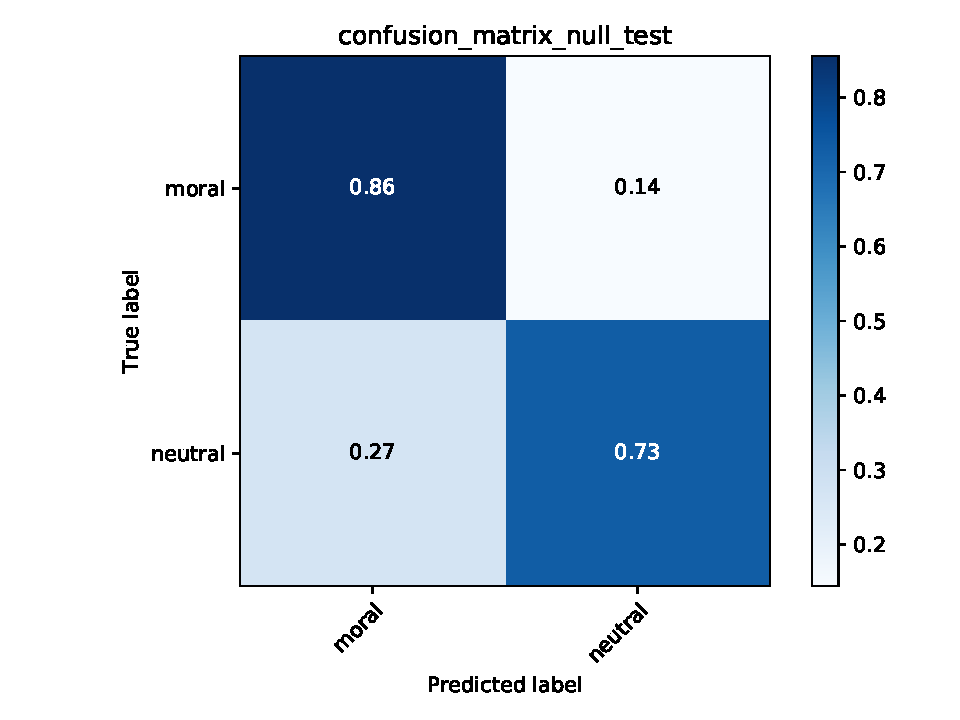
\includegraphics[width=1.5\linewidth]{confusion-matrix-centroid-fixed-seeds/confusion_matrix_null_test.pdf}
    \caption{Null test confusion matrix for fixed seeds.}
    \label{fig:confusion-null-fixed}
\end{figure}

\begin{figure}[H]
    \centerfloat
    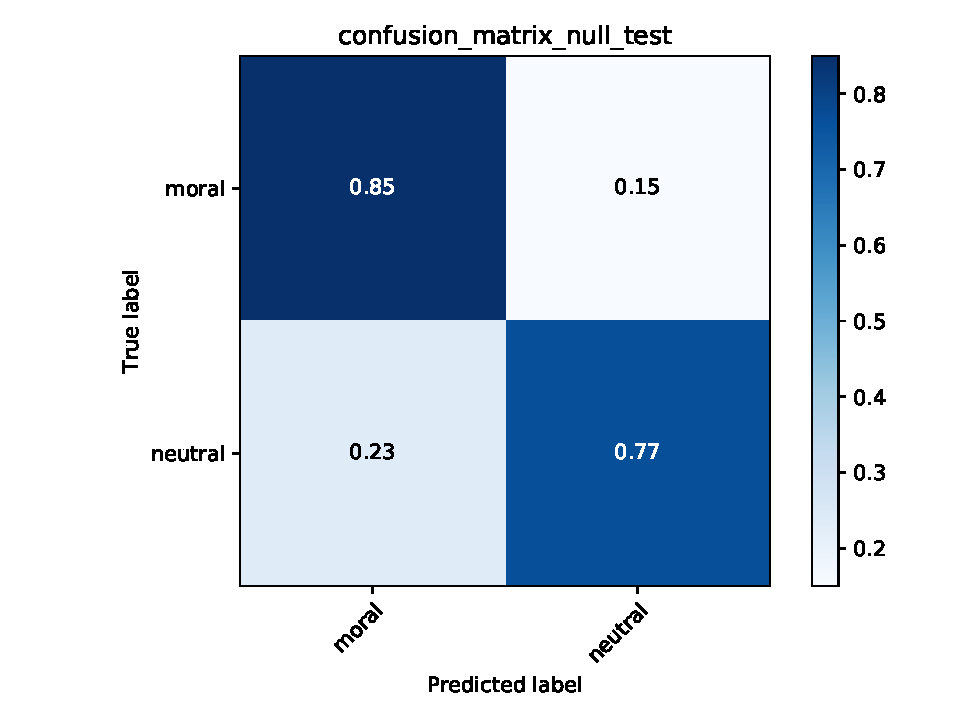
\includegraphics[width=1.5\linewidth]{confusion-matrix-centroid-varying-seeds/confusion_matrix_null_test.pdf}
    \caption{Null test confusion matrix for varying seeds.}
    \label{fig:confusion-null-varying}
\end{figure}

\begin{figure}[H]
    \centerfloat
    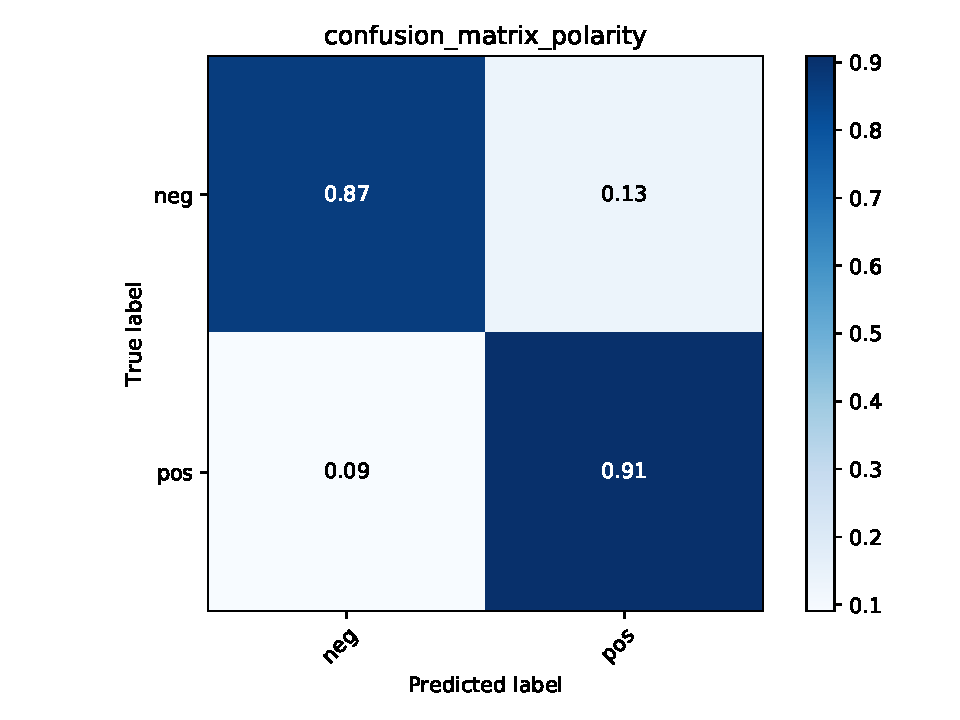
\includegraphics[width=1.5\linewidth]{confusion-matrix-centroid-fixed-seeds/confusion_matrix_polarity.pdf}
    \caption{Polarity test confusion matrix for fixed seeds.}
    \label{fig:confusion-polarity-fixed}
\end{figure}

\begin{figure}[H]
    \centerfloat
    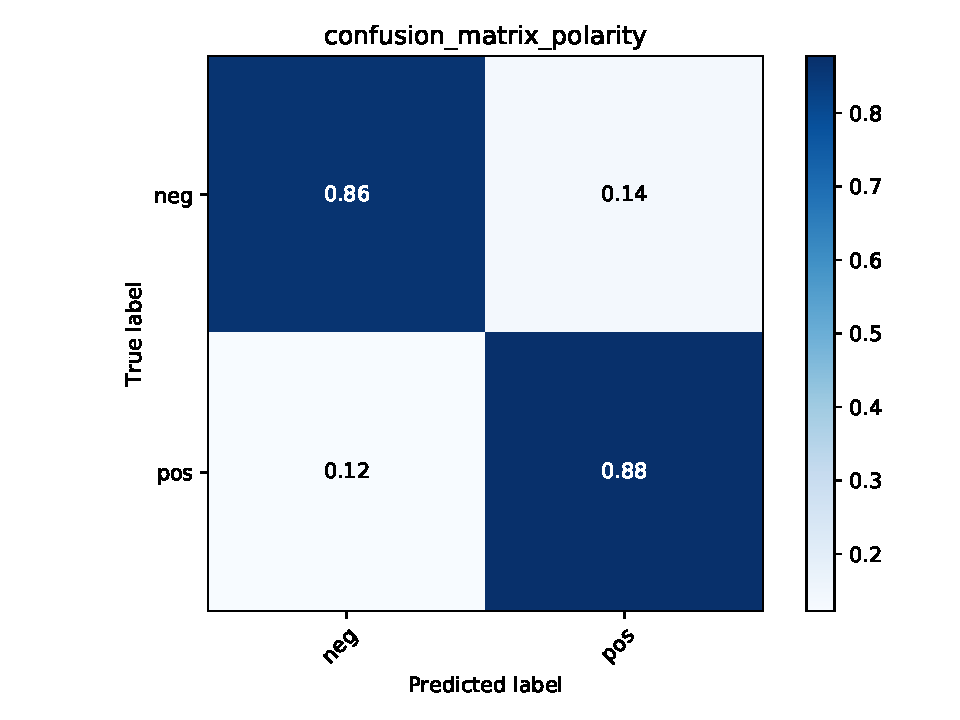
\includegraphics[width=1.5\linewidth]{confusion-matrix-centroid-varying-seeds/confusion_matrix_polarity.pdf}
    \caption{Polarity test confusion matrix for varying seeds.}
    \label{fig:confusion-polarity-varying}
\end{figure}

\begin{table}[H]
    \centering
    \caption{Sizes of seed word sets per class in fixed and varying regimes.}
    \begin{tabular}{c | c | c}
        \textbf{category}   & \textbf{fixed seeds} & \textbf{varying seeds} \\ \hline
        +authority &    40       &     54        \\
        +care      &    18       &     27        \\
        +fairness  &    18       &     26        \\
        +loyalty   &    16       &     30        \\
        +sanctity  &    21       &     33        \\ \hline
        -authority &    18       &     32        \\
        -care      &    28       &     33        \\
        -fairness  &    12       &     23        \\
        -loyalty   &    7        &     16        \\
        -sanctity  &    30       &     53        \\ \hline
        pos        &    113      &     170       \\
        neg        &    95       &     157       \\ \hline
        moral      &    208      &     327       \\
        neutral    &    67       &     151       \\
    \end{tabular}
    \label{tab:sizes}
\end{table}

\section{Prediction errors}

\Cref{tab:errors-fixed,tab:errors-varying} show the mistakes made by the
model in leave-one-out classification across all tasks in the decade of 1990,
in the fixed seeds and varying seeds regimes, respectively.

\Cref{tab:errors-fixed-1800,tab:errors-varying-1800} show the same data
for the decade of 1800.

\csvautobooklongtable[respect underscore=true,
table head ={
\caption{Prediction errors of centroid model on fixed seeds regime in 1990.}\\
\hline\csvlinetotablerow\\\hline
\label{tab:errors-fixed}
}]{errors_centroid_fixed_seeds_1990.csv}

\csvautobooklongtable[respect underscore=true,
table head={
\caption{Prediction errors of centroid model on varying seeds regime in 1990.}\\
\csvlinetotablerow\\\hline
\label{tab:errors-varying}
}]{errors_centroid_varying_seeds_1990.csv}

\csvautobooklongtable[respect underscore=true,
table head ={
\caption{Prediction errors of centroid model on fixed seeds regime in 1800.}\\
\hline\csvlinetotablerow\\\hline
\label{tab:errors-fixed-1800}
}]{errors_centroid_fixed_seeds_1800.csv}

\csvautobooklongtable[respect underscore=true,
table head={
\caption{Prediction errors of centroid model on varying seeds regime in 1800.}\\
\csvlinetotablerow\\\hline
\label{tab:errors-varying-1800}
}]{errors_centroid_varying_seeds_1800.csv}

\end{document}
